\chapter{Farmacocinetica}

La curva dose/concentrazione di un farmaco si basa su una media del funzionamento del farmaco. Ma questa curva può variare di molto da individuo a individuo.

I due parametri principali che influenzano questa variabilità sono il \textbf{volume di distribuzione} e la \textbf{cleareance}.

\section{Volume di distribuzione}

\`E quel volume teorico che contiene quella determinata concentrazione di farmaco nel comparto in oggetto, spesso il flusso sanguigno

$$V =\frac{\text{quantità di farmaco nell'organismo}}{[F]}$$

ove $[F]$ può essere riferito a sangue, plasma, farmaco libero.

Come si vede dalla relazione $V$ è uno spazio virtuale in quanto si presuppone che la concentrazione misurata in $[F]$ sia omogenea su tutto il corpo.

Quindi farmaci con distribuzione prettamente ematica danno delle $V$ piccole e confrontabili con il valore reale del compartimento che, per il sangue, è $\simeq 3\ce{L}/70\ce{Kg}$.

Farmaci con distribuzione prettamente extravascolare avremo piccole concentrazioni nel sangue e quindi $V$ elevati. Ad esempio, per la digossina, $V \simeq 500\ce{L}/70\ce{Kg}$.

La $V$ è utile, ad esempio, nel calcolo dell'emivita come vedremo a breve.

\section{Clereance}

\`E la quantità di farmaco eliminata nel tempo in rapporto alla sua concentrazione nel comparto in oggetto (sangue, plasma, farmaco libero)

$$CL =\frac{\text{velocità di eliminazione}}{[F]}$$

La clearenace è additiva per cui se un farmaco ha eliminazione renale, epatica e respiratoria

$$ CL_{tot} = CL_{\text{rene}} + CL_{\text{epat.}} + CL_\text{resp.} = \frac{V_{\text{rene}}^{\text{elim}}}{[F]} + \frac{V_{\text{epat.}}^{\text{elim}}}{[F]} + \frac{V_{\text{resp}}^{\text{elim}}}{[F]}$$

Per la maggior parte dei farmaci la clereance è costante all'interno del range di concentrazioni della pratica terapeutica per cui la velocità di eliminazione dipende solo dalla concentrazione del farmaco

$$\ce{Vel.} = CL \cdot [F]$$

Quando ciò accade si parla di cinematica di ordine 1. In questo caso la clereance può essere calcolata misurando l'area sotto la curva (AUC) delle concentrazioni ematiche nel tempo dopo somministrazione di una singola dose di farmaco come

$$\text{CL} = \frac{\text{dose}}{\text{AUC}}$$

\section{Eq. di Michaelis--Menten}

Ma non tutti i farmaci seguono un andamento lineare. Alcuni farmaci (\index{fenitoina}fenitoina, \index{etanolo}etanolo, \index{acido acetilsalicilico}acido acetilsalicilico) hanno un'eliminazione saturabile a cinematica non lineare.

Questi seguono l'equazione di Michaelis--Menten

$$v_{\text{elim}} = \frac{v_{\text{max}}\cdot [F]}{K_m + [F]}$$

dove $K_m$ è chiamata costante di Michaelis--Menten e rappresenta la concentrazione del farmaco che produce una velocità di eliminazione del 50\% della massima.

A concentrazioni levate la $v_{\text{elim}}$ non dipende più dalla concentrazione e diventa costante con una cinetica di ordine 0. 

Per questi farmaci non si può parlare di clereance ne usare l'AUC per descrivere la loro eliminazion.

\section{Emivita}

L'emivita di un farmaco è definita come il tempo necessario a ridurre
il farmaco a \unitfrac{1}{2} della quantità di farmaco presente nell'organismo
allo steady-state.

Supponendo un modello monocorpartimentale, la variazione della concentrazione nel tempo è una funzione lineare della concentrazione stessa

$$\frac{d\,q}{d\,t} = -kq$$

che ha come soluzione una esponenziale decrescente con il tempo:

$$
q(t)=q_0 e^{-kt}
$$

con $q_0$ concentrazione iniziale. Per calcolare il parametro $k$ valutiamo la AUC di questo andamento

$\text{AUC} =\displaystyle\int_0^\infty q_0e^{-kt}\,dt = \frac{q_0}{k}$ ma d'altra parte $\text{AUC} = \displaystyle\frac{\text{dose}}{\text{CL}}$ ed essendo 

$\text{dose} = Vq_0$ si ha che $\displaystyle\frac{Vq_0}{\text{CL}} = \frac{q_0}{k} \Rightarrow k = \frac{\text{CL}}{V}$ e quindi

$$q(t) = q_0\,e^{-\frac{\text{CL}}{V}t}$$

e ponendo $q(t_{\unitfrac{1}{2}}) = \displaystyle\frac{q_0}{2}$ si ha che

$$t_{\unitfrac{1}{2}}=\ln\,2\cdot\dfrac{V}{\text{CL}}\simeq0.7\cdot\dfrac{V}{\text{CL}}$$

Identica curva, ma al contrario, per l'accumulo durante una somministrazione continua a velocità costante.

Così, dopo $t_{\unitfrac 12}$ avrò il 5\% di $q_0$ e dopo circa 4 emivite avrò più del 90\% del $q_0$.

Analogamente nell'eliminazione, dopo 4 emivite, avrò meno del 10\% del farmaco iniziale nel corpo.

Nel caso di somministrazioni multiple, se l'intervallo tra le dosi è minore di 4 emivite avrò un accumulo di farmaco e questo accumulo è inveramente proporzionale alla frazione di farmaco eliminata

$$\text{frazione di accumulo} = \frac{1}{\text{frazione di farmaco eliminato}} = \frac{1}{1-\text{frazione residua}}$$

cosi, ad esempio, un farmaco somministrato ogni emivita ha una frazione di accumulo pari a $\frac{1}{0.5} = 2$.

\section{Biodisponibilità}

\`E la frazione di farmaco non modificato che raggiunge la circolazione sistemica

\begin{tikzpicture}
	\Tree
	[.{vie di somministrazione}
		[.{endovenosa (IV)}
			{bio: 100\%}
		]
		[.{intramuscolare (IM)}
			{bio: $75\sim \leq 100$}
		]
		[.{sottocutanea (SC)}
			{bio: $75\sim \leq 100$}
		]
		[.{orale (PO)}
			{bio: $5\sim < 100$}
		]
		[.{rettale (PR)}
			{bio: $30\sim < 100$}
		]
		[.{inalatoria}
			{bio: $5\sim < 100$}
		]
		[.{transdermica}
			{bio: $80\sim \leq 100$}
		]															
	]
\end{tikzpicture}

\section{Effetto di primo passaggio}

A seguito dell'assorbimento per os il farmaco attraversa il fegato prima di andare nella circolazione sistemica e qui può perdere una frazione $\text{ER}$ di quanto assorbito $f$ con un valore di biodisponibilità $F$ pari a 

$$F=f(1-\text{ER})$$
dove $\text{ER} = \displaystyle\frac{\text{CL}_{\text{fegato}}}{\Phi^{\text{fegato}}_{\text{ematico}}}$ con $\Phi\simeq 90$L/h/70Kg.

Ad esempio, la morfina è quasi tutta assorbita nell'intestino per cui $f=1$. Tuttavia la $\text{CL}_{\text{fegato}}^{\text{morfina}} = 60$L/h/70Kg cosi che $\text{ER}=0.67$ da cui la biodisponibilità orale della morfina è $\simeq 0.33$.

\section{Dose di mantenimento}

I farmaci vengono somministrati per mantenere quanto più possibile uno stato stazionario ad un livello di concentrazione target $[F]_\text{target}$ andando a compensare l'eliminazione del farmaco. A regime quindi

$$v_\text{somm} = v_\text{elim} = \text{CL}\cdot[F]_\text{target}$$

e, se la via di somministrazione non è quella ideale ma, ad esempio, quella orale

$$v_\text{somm}^\text{orale} = \frac{v_\text{somm}}{[F]_\text{orale}}$$

Se invece di una somministrazione continua ho dosi ripetute, la dose di mantenimento è tale che 

$$\text{dose}_\text{mant} = v_\text{somm} \cdot \text{intervallo tra le dosi}$$

Se l'emivita del farmaco è lunga e quindi lo stato stazionario lo raggiungerei dopo molto tempo si può somministrare una dose di carico per raggiungere brevemente la concentrazione target come

$$\text{dose}_\text{carico} = V_\text{DIST} \cdot [F]_\text{target}$$



